\chapter{Introduction}
\label{Introduction}

	Differential equations, ordinary or partial, allow modeling phenomena that evolve with respect to space and time. They are commonly used to describe the propagation of sound or heat and appear frequently in models related to electrostatics, electrodynamics, fluid dynamics, elasticity, quantum mechanics, and among other more related areas. \\
	
	However, their analytical solutions cannot always be easily obtained and in many cases, it will be necessary to resort to very complex techniques that tend to give solutions with very impractical mathematical expressions to use. In particular, problems characterized as non-linear present these difficulties, and considering a different alternative to find solutions may be a more reasonable option. \\  
	
	There are alternatives to find solutions to differential equations, which depend on the nature of the problem to be solved. For example, computational fluid dynamics is one of the branches of fluid mechanics that uses numerical methods and algorithms to solve and analyze fluid flow problems that perform millions of calculations to simulate the interaction of liquids and gases through complex surfaces. However, even with simplified equations and high-performance supercomputers, in many cases, only approximate results can be achieved. \\
	
	The resolution of differential equations related to the characterization of fluids, and in general, for those that occur in the field of complex systems, are considered of utmost importance since they allow studying problems of great interest such as the turbulence phenomenon that allows understanding with precision its dynamics. Understanding these phenomena through differential equations is not enough, it is also necessary to characterize their nature, which in some cases is possible if the dimensionless value of the Reynolds number ($Re$) that indicates whether a fluid follows a laminar flow is known or turbulent. However, it is not always possible to predict with this information those phenomena that present turbulence in a combination of convection or combustion processes, and that therefore require greater attention in their dynamics. \\
	
	Spectral methods have recently emerged as a viable alternative for the numerical solution of partial differential equations. They have proved particularly useful in fluid dynamics simulation where are now regularly used large spectral hydrodynamics codes to study turbulence, numerical weather prediction, ocean dynamics, and any other problems where high accuracy is desired. \\
	
	Due to the above, he has motivated the development of this thesis by studying spectral methods extensively to acquire the ability to use this tool and understand them from the point of view of mathematical analysis. To develop this study we will focus first on the elementary theory of these methods, encompassing enough knowledge to allow us to develop, implement and analyze under this approach a wide variety of problems that arise in the partial differential equations that evolve. \\
	
	To understand the application of these methods, the well-known Burgers' equation has been considered, since it is an ideal problem for understanding these methods because, in addition to being a non-linear problem that presents interesting characteristics, it can be useful to develop the ability to attack more complex problems. Furthermore, in order to extend the study of the implementation of spectral methods, we are going to work with the stochastic version of this equation that will be very useful for us to know in general terms trying to solve problems of this type, which are considered of great importance for its wide field of applications and that it is still an area that is in full development due to the great difficulty in obtaining solutions. \\
	
	To carry out this study, we will divide the work into six parts organized as follows
	\begin{enumerate}
		\item[1.] In chapter \ref{Introduction}, a brief history of Burgers' equation will be presented in its deterministic version, and we will also present how to obtain the analytical solution for an initial value problem of this equation, transforming it into another linear one that can be solved using the Fourier transform. Later, the origin of the stochastic version will be discussed, in addition to its importance within mathematics and physics.
		
		\item[2.] In chapter \ref{Chapter_2}, we will study the theoretical bases of spectral methods using the well-known Fourier series as the main tool, which will allow us to study a theory of approximation of functions under two approaches, using orthogonal projections and another using interpolation techniques. These two approaches will be examined independently, studying their implementation and some theoretical results that will be useful in chapter \ref{Chapter_3}.  
		
		\item[3.] In chapter \ref{Chapter_3}, the spectral methods known as Fourier-Galerkin and Fourier-Collocation will be developed using the tools examined in chapter \ref{Chapter_2}, verifying their convergence theory. For this, the deterministic Burgers' equation will be used, taking advantage of its linearized form to describe the methods, which will then be applied to the original nonlinear equation to describe the algorithms of its computational implementation that will allow us to perform numerical experiments and to be able to observe some characteristics interesting for your discussion.
		
		\item[4.] In chapter \ref{Chapter_4}, a spectral method used to solve stochastic partial differential equations that was studied in \cite{Delgado2016} will be disclosed in as much detail as possible. We will see that this method, which is built based on the well-known Hermite polynomials, will allow us to obtain solutions of stochastic problems by solving a deterministic type problem, and will be illustrated using the stochastic Burgers' equation developing its implementation and also numerical simulations.
		
		\item[5.] In this last chapter, we will discuss the most relevant of each chapter, and we will give some observations of the obtained numerical results to conclude with some ideas that can be considered to extend this work.
		
		\item[6.] At the end of this work, an appendix \ref{Appendix_A} was added, which will be useful to understand in more detail the spectral method developed in chapter \ref{Chapter_4}.
	\end{enumerate}
	
	\section{Brief History of Burgers' Equation}
    
    The simplest fluids (called Newtonian fluids), are described by the well-known Navier-Stokes equations, named after Claude-Louis Navier and George Gabriel Stokes. These are a set of non-linear (PDEs), which are obtained by applying the principles of conservation of mechanics and thermodynamics on a volume of fluid to obtain the so-called integral formulation of the equations. Applying certain considerations, especially those in which the tangential forces have a linear relationship with the velocity gradient (Newton's viscosity law), the differential formulation is obtained which is generally more useful for solving the problems that arise in the mechanics of fluids. For further details about the Navier-Stokes equations see \cite{Acheson2001, Batchelor1967, Landau1987, Currie1974, Temam1984}. \\
    
    Let $v$ be a vector field, Navier-Stokes equations are given as follows
    \begin{equation}
        \left \lbrace \begin{array}{ll}
    	\nabla \cdot v = 0, \\
    	(\rho v)_t + (\nabla \cdot \rho v) v + \nabla p - \mu \nabla^2 v - \rho G = 0.
    	\end{array}  \right .
    	\label{navierstokes}
    \end{equation}
    It is well known that when $\rho$ is considered the density, $p$ the pressure, $v$ the velocity and $\mu$ the viscosity of a fluid, these equations describe the dynamics of an incompressible fluid (free divergence, and $\rho_t = 0$), where $G$ represents the gravitational effects. \\
    
    In contrast to equation (\ref{navierstokes}), this can be investigated in one spatial dimension. Simplification in (\ref{navierstokes}) of the $x$ component of the velocity vector, which we will call $v^x$, gives
    \begin{equation*}
        \rho \frac{\partial v^x}{\partial t} + \rho v^x \frac{\partial v^x}{\partial x} + \rho v^y \frac{\partial v^x}{\partial y} + \rho v^z \frac{\partial v^x}{\partial z} + \frac{\partial p}{\partial x} - \mu \left(\frac{\partial^2 v^x}{\partial x^2} + \frac{\partial^2 v^x}{\partial y^2} + \frac{\partial^2 v^x}{\partial z^2} \right) - \rho G^x = 0.
    \end{equation*}

    \noindent Considering a $1D$ problem with no pressure gradient, the above equation reduces to\\
    \begin{equation}
        \rho \frac{\partial v^x}{\partial t} + \rho v^x \frac{\partial v^x}{\partial x} - \mu \frac{\partial^2 v^x}{\partial x^2} - \rho G^x = 0.
        \label{1.2}
    \end{equation}
    If we use now the traditional variable $v$ rather than $v^x$, take $\alpha$ to be the kinematic viscosity, i.e, $\alpha = \frac{\mu}{\rho}$ and $G \equiv 0$, then the equation (\ref{1.2}) becomes just the viscid Burgers' equation
    \begin{equation}
    \label{Burgers_Equation}
        \frac{\partial v(x, t)}{\partial t} +  \underbrace{v(x, t) \frac{\partial v(x, t)}{\partial x}}_{\textbf{Convection}} - \underbrace{\alpha \frac{\partial^2 v(x, t)}{\partial x^2}}_{\textbf{Diffusion}} = 0.
    \end{equation}

    Some assumptions  are  made,  namely: $\rho =$ constant (density), $\mu =$ constant  (viscosity),  $p=$ constant (pressure). \\
    
    Burgers' equation was introduced in 1915 by Harry Bateman \cite{Bateman1915}, an English mathematician, in his paper along with its corresponding initial condition and boundary values. Later in 1939, Johannes Martinus Burgers \cite{Burgers1939,Burgers1948}, a Dutch physicist, simplified the Navier-Stokes equation (\ref{navierstokes}) by just dropping the pressure term, and in 1948 explained the  mathematical modeling of turbulence with the help of the equation (\ref{Burgers_Equation}). The name of this equation is because Burgers became one of the leading figures in the field of fluid mechanics and, therefore, honors his contributions. \\  
    
    The equation (\ref{Burgers_Equation}) is a partial differential equation nonlinear, where the second term is known as the convective part of the equation and the third as the diffusive part. This equation appears in several areas of applied mathematics, such as fluid mechanics, nonlinear acoustics, gas dynamics, traffic flow, and many others. It is generally considered a toy model, i.e., a tool that is used to understand part of the internal behavior of the general problem.  \\
    
    The formulation given by the equation (\ref{Burgers_Equation}) is called the strong form, i.e., the partial differential equation requires that it be satisfied for each point $x$ in its domain and for each $t$. This formulation can be written as follows
    \begin{equation}
    	\frac{\partial v}{\partial t} + A(v) + F(v) = 0, \hspace{2mm} t > 0,
    	\label{strong}
    \end{equation}
	where $F$ and $A$ are given by
	\begin{equation*}
		A(v) = - \alpha v_{xx}, \hspace{3mm} F(v) = \frac{1}{2} (v^2)_x , \hspace{3mm} x \in I.
	\end{equation*} 
	Multiplying both sides of (\ref{strong}) by $\phi \in X$, for some arbitrary smooth function $\phi$ of compact support, such that the integral of the PDE over the space $I$ is satisfied, we get   
    \begin{equation}
    	\displaystyle \int_{I} \frac{\partial v}{\partial t} \phi dx + \int_{I} A(v) \phi dx + \int_{I} F(v) \phi dx = 0, \hspace{2mm} \forall \phi \in X,\hspace{2mm} \forall t > 0.
    	\label{weak}
    \end{equation}
	The formulation (\ref{weak}) is called the weak form of (\ref{Burgers_Equation}) and $\phi$ are known as the test functions.  If we denote $\langle \cdot, \cdot \rangle$ as the inner product in $X$, then (\ref{weak}) can be written in compact form as follows
    \begin{equation}
    	\left \langle \frac{\partial v}{\partial t} + A(v) + F(v), \phi\right\rangle = 0, \hspace{2mm} \forall \phi \in X, \hspace{2mm} \forall t > 0.	
    	\label{compact_weak}
    \end{equation}
	Note that the two formulations, (\ref{weak}) and (\ref{strong}), are equivalent if the solution is smooth enough, however the weak formulation can adjust less regular solutions than in the strong form. In fact, the solution to (\ref {weak}) is known as the distribution solution of the original equation (\ref{Burgers_Equation}), since it can be shown to satisfy (\ref{Burgers_Equation}) in the sense of distributions. For more details of the above it is recommended to see Schwartz \cite{Schwartz1966}, Lions and Magenes \cite{Lions1972}, Renardy and Rogers \cite{Renardy1993}. \\
	
	Proper use of these formulations allows one to recover the strong form from the weak form, therefore, an appropriate way to design a numerical method is to first choose one of the formulations satisfied by the exact solution, then restrict the choice of test functions to a space of finite dimension, to replace $u$ with the discrete solution $u_N$, and possibly to replace the exact integration with quadrature rules. \\
	
   
    \subsection{Analytical solutions for Burgers' equation.}
    
    When we want to know the precision of an approximation, an alternative is through numerical experiments that can be compared with some other solution considered as a good reference. For this type of tests, the better is to have exact solutions to compare with an approximate one, and fortunately the equation (\ref{Burgers_Equation}) can be solved exactly by Hopf-Cole transformation introduced by Eberhard Hopf \cite{Hopf1950} and Julian David Cole \cite{Cole1951} independently to convert the Burgers' equation into a linear parabolic equation and solve it exactly for any initial condition. \\
  
   	\noindent Now consider the problem of initial value for the equation (\ref{Burgers_Equation}) as follows
    \begin{equation}
        \left \lbrace \begin{array}{ll}
    	u_t + u u_x = \alpha u_{xx} & x \in \mathbb{R}, \hspace{2mm} t > 0, \hspace{2mm} \alpha > 0 \\
    	u (x, 0) = u_0 (x)  & x \in \mathbb{R},
    	\end{array}  \right .
    	\label{IVP}
    \end{equation}
	Hence, the transformation known as the Cole-Hopf transformation is given by
    \begin{equation}
        u = -2 \alpha \frac{\varphi_x}{\varphi}
        \label{Hopf_tranform}
    \end{equation}
    Operating (\ref{Hopf_tranform}) into each term of (\ref{IVP}) we find that
    \begin{equation*}
        u_t = \frac{2 \alpha (\varphi_t \varphi_x - \varphi \varphi_{x t})}{\varphi^2} \hspace{2mm} , \hspace{2mm} u u_x = \frac{4 \alpha^2 \varphi_x (\varphi \varphi_{xx} - \varphi^2_x)}{\varphi^3},
    \end{equation*}
    and 
    \begin{equation*}
        \alpha u_{xx} = - \frac{2 \alpha^2 (2 \varphi_x^3 - 3 \varphi \varphi_{xx} \varphi_x + \varphi^2 \varphi_{xxx})}{\varphi^3}.
    \end{equation*}
    Substituting these expressions into (\ref{IVP}),
    \begin{align*}
        \frac{2 \alpha (-\varphi \varphi_{x t} +  \varphi_x ( \varphi_t - \alpha \varphi_{xx}) + \alpha \varphi \varphi_{xxx})}{\varphi^2} = 0, 
    \end{align*}
	so we have the following,
	\begin{align*}    
        - \varphi \varphi_{x t} + \varphi_x (\varphi_t - \alpha \varphi_{xx}) + \alpha \varphi \varphi_{xxx} = 0 &\Longleftrightarrow \varphi_x (\varphi_t - \alpha \varphi_{xx}) = \varphi (\varphi_{x t} - \alpha \varphi_{xxx}) \\
        &\Longleftrightarrow \varphi_x (\varphi_t - \alpha \varphi_{xx}) =  \varphi (\varphi_t - \alpha \varphi_{xx})_x.
    \end{align*}
    Therefore, if $\varphi$ solves the equation $\varphi_t - \alpha \varphi_{xx} = 0$, $x \in \mathbb{R}$, then $u(x, t)$ given by the transformation (\ref{Hopf_tranform}) solves the Burgers equation.\\
    
    \noindent To completely transform the problem (\ref{IVP}) we still have to work with the initial condition function. To do this, note that (\ref{Hopf_tranform}) can be written as
    \begin{equation}
        u = -2 \alpha (\log \varphi)_x,
        \label{Hopf2}
    \end{equation}
    
    \noindent hence, we get
    \begin{equation*}
        \varphi (x, t) = \displaystyle e^{- \int \frac{u(x, t)}{2 \alpha} dx}.
    \end{equation*}
    It is clear from (\ref{Hopf2}) that multiplying $\varphi$ by a constant does not affect $u$, so we can write the last equation as
    \begin{equation}
        \varphi (x, t) = \displaystyle e^{- \int_{0}^{x} \frac{u(y, t)}{2 \alpha} dy}.
        \label{phi}
    \end{equation}
    The initial condition on (\ref{IVP}) must be transformed by using (\ref{Hopf2}) to get
    \begin{equation*}
        \varphi (x, 0) = \varphi_0 (x) = \displaystyle e^{- \int_{0}^{x} \frac{u_0 (y)}{2 \alpha} dy}.
    \end{equation*}
    In summary, we have reduced the problem (\ref{IVP}) to this one
    \begin{equation}
        \left \lbrace \begin{array}{ll}
    	\varphi_t - \alpha \varphi_{xx} = 0,  & x \in \mathbb{R}, \hspace{2mm} t > 0, \hspace{2mm} \alpha > 0, \\
    	\varphi (x, 0) = \varphi_0 (x) = \displaystyle e^{- \int_{0}^{x} \frac{u_0 (y)}{2 \alpha} dy}, & x \in \mathbb{R}.
    	\end{array}  \right .
    \label{heat}
    \end{equation}
    \paragraph{Parabolic Equation.} The general solution of the initial value problem for the equation (\ref{heat}) is well known and can be handled by a variety of methods. An interesting method related to spectral methods is the following: one can take the Fourier transform with respect to $x$ for both the equation and the initial condition $\varphi_0 (x)$ to obtain a first-order (ODE) as follows
    \begin{equation*}
        \left \lbrace \begin{array}{ll}
    	\hat{\varphi}_t = \xi^2 \alpha \hat{\varphi},  & \xi \in \mathbb{R}, \hspace{2mm} t > 0, \hspace{2mm} \alpha > 0, \\
    	\hat{\varphi} (\xi, 0) = \hat{\varphi}_0 (\xi), & \xi \in \mathbb{R},
    	\end{array}  \right .
    \end{equation*}
    where $\hat{\varphi} (\xi, t) = \displaystyle \int_{-\infty}^{\infty} \varphi (x, t) e^{i \xi x} dx $. \\
    
    \noindent Then the solution for this problem is
    \begin{equation*}
         \hat{\varphi} (\xi, t) =  \hat{\varphi}_0 (\xi) e^{ \xi^2 \alpha t}.
    \end{equation*}
    
    \noindent To recover $\varphi (x, t)$ we have to use the inverse Fourier transformation $F^{-1}$ , namely,
    \begin{equation*}
        \varphi (x, t) = F^{-1} (\hat{\varphi} (\xi, t)) = F^{-1} (\hat{\varphi}_0 e^{\xi^2 \alpha t}) = \varphi_0 (x) \ast F^{-1} (e^{\xi^2 \alpha t}),
    \end{equation*}
    where $\ast$ denotes the convolution product.\\
    
    \noindent On the other hand
    \begin{equation*}
        F^{-1} (e^{\xi^2 \alpha t}) = \frac{1}{2 \sqrt{\pi \alpha t}} e^{- \frac{x^2}{4 \alpha t}},
    \end{equation*}
    so the initial value problem (\ref{heat}) has the analytic solution
    \begin{equation*}
        \varphi (x, t) = \frac{1}{2 \sqrt{\pi \alpha t}} \displaystyle \int_{-\infty}^{\infty} \varphi_0 (\xi) e^{- \frac{(x - \xi)^2}{4 \alpha t}} d\xi.
    \end{equation*}
    Finally, from (\ref{Hopf_tranform}), we obtain the analytic solution for the problem (\ref{IVP})
    \begin{equation}
    \label{Exact_Solution}
        u (x, t) =  \displaystyle \frac{\int_{-\infty}^{\infty} \frac{x - \xi}{t} \varphi_0 (\xi) e^{- \frac{(x - \xi)^2}{4 \alpha t}} d\xi}{\int_{-\infty}^{\infty} \varphi_0 (\xi) e^{- \frac{(x - \xi)^2}{4 \alpha t}} d\xi}. 
    \end{equation}
    
    However, the previous solution cannot always be calculated explicitly and we must implement some numerical integration method very efficiently to obtain a good approximation.
    
    \begin{figure}[H]
    	\centering
    	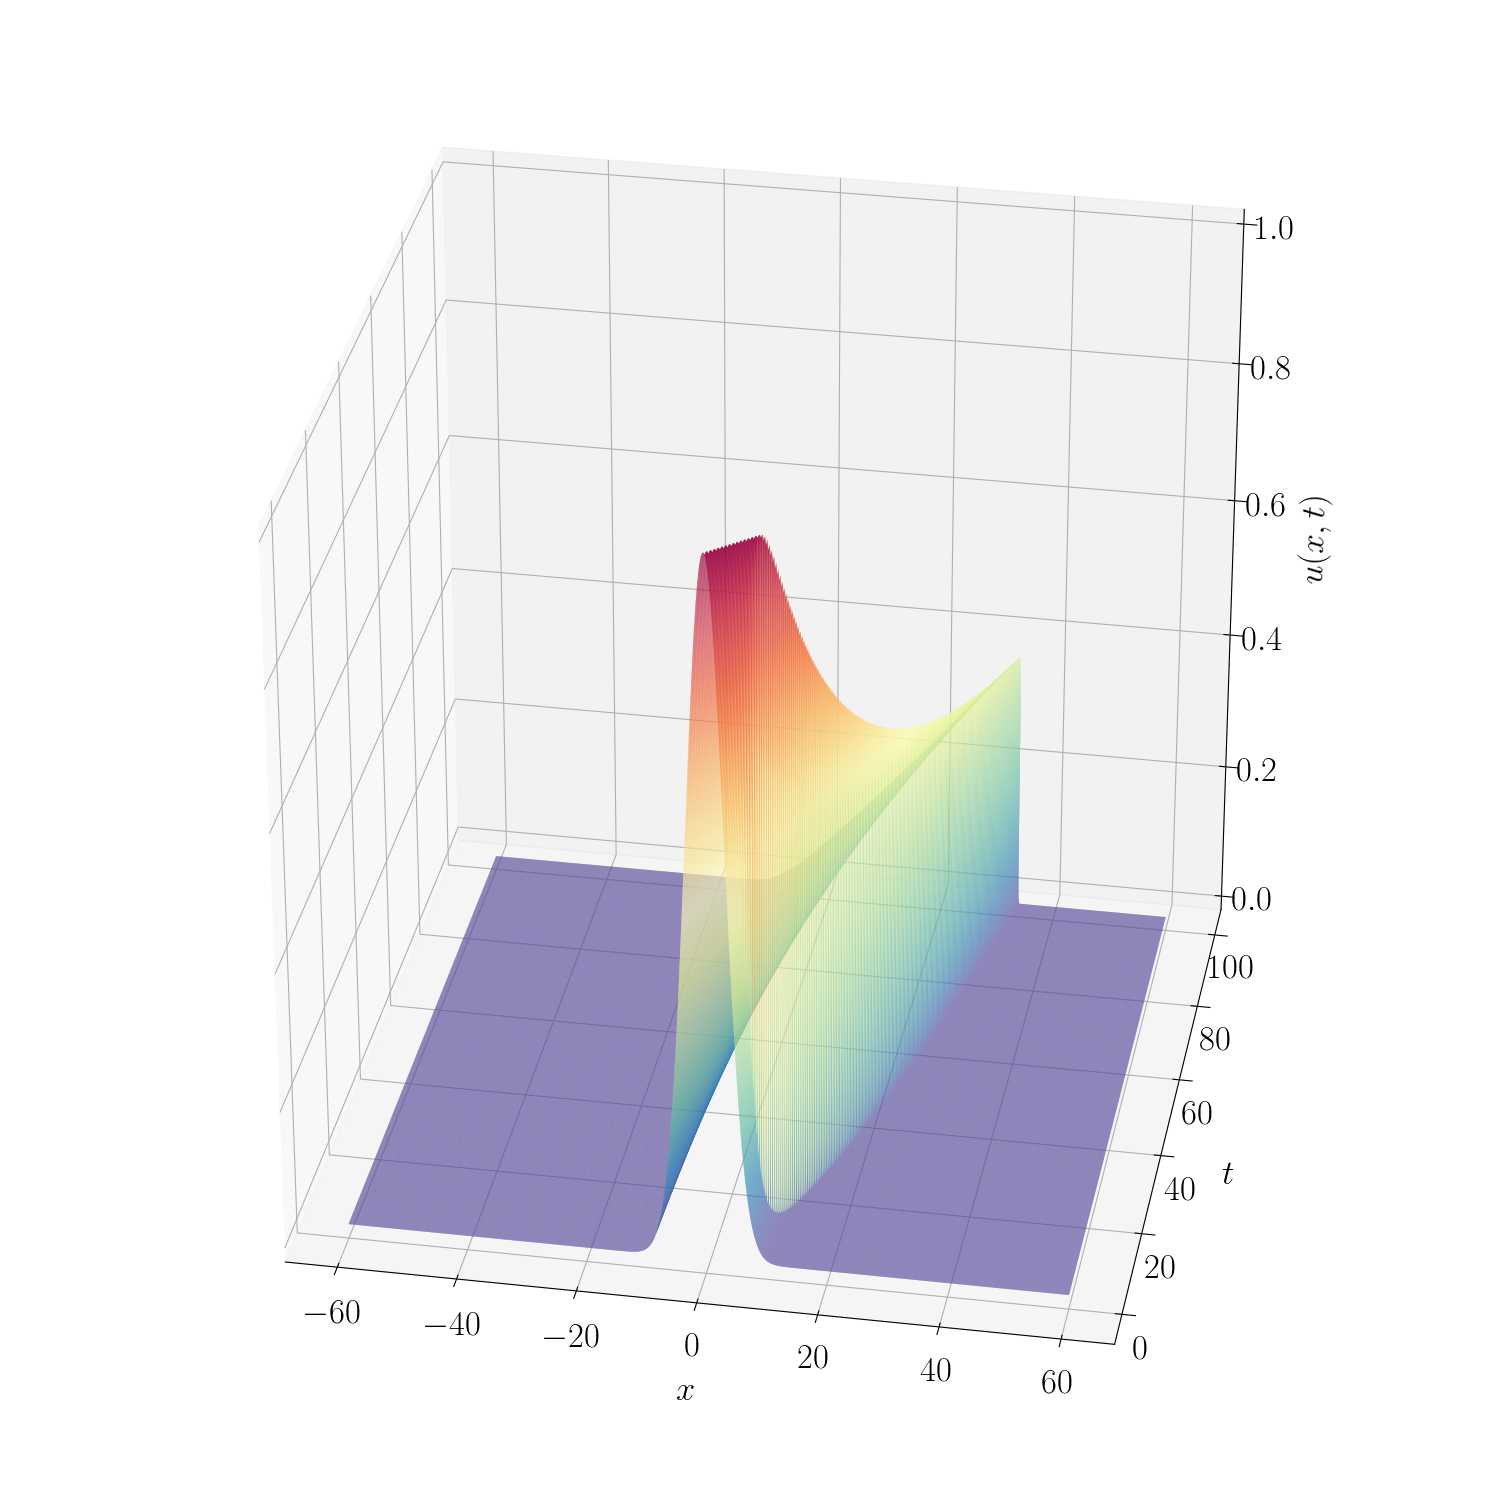
\includegraphics[width=11cm]{introduction/figures/Exact_Solution_alpha=001.png}
    	\caption{Exact solution for (\ref{IVP}) with initial condition $u_0 (x) = e^{-0.05x^2}$ using the equation (\ref{Exact_Solution}) for $x \in [-60, 60]$, $t \in [0, 100]$, and $\alpha = 0.01$.}
    	\label{Exact_Solution_alpha=0.01}
    \end{figure}
	\newpage
	\section{The Stochastic Burgers' equation}
     
    In real situations, the mathematical modeling of physical phenomena in a deterministic manner does not always produce satisfactory results, since certain hypotheses are established for their formulation, increasing uncertainty regarding spatial or temporal variables. To predict the behavior of a fluid, it is necessary to calculate the exact trajectory of each of the particles that compose it (which is an unapproachable problem). 
    
    When a fluid is in a closed container under pressure, each particle gets pushed against by all the surrounding particles. The container walls and the pressure-inducing surface (such as a piston) push against them in (Newtonian) reaction. These macroscopic forces are actually the net result of a very large number of intermolecular forces and collisions between the particles in those molecules. One fluid flow is isotropic if there is no directional preference (e.g. in fully developed turbulence); the kinetic theory of gases is also an example of isotropy if it's assumed that the molecules move in random directions and as a consequence, there is an equal probability of a molecule moving in any direction. 
    
    The equation given by (\ref{navierstokes}) assumes that the fluid is incompressible and isotropic, where the viscous stress is given by a linear relationship with the velocity gradient (Newton's viscosity law). In addition, the collective behavior of the fluid depends only on a few macroscopic variables (such as pressure, volume, and temperature) where the internal structure of the system and the individual behavior of the particles is not relevant for thermodynamic quantities. 
    
    Sometimes, due to the large size of such a system, quantum effects can be ignored and Newton's laws may be a good approximation (in some cases, if particles move very quickly with relativistic mechanics). But it is also possible to model a fluid as a set of randomly displaced point particles that do not interact with each other, analyzed by statistical mechanics.
    
    The information necessary to specify a physical system has to do with its entropy. When energy is degraded, Boltzmann said, it is because atoms assume a more disorderly state. And entropy is a parameter of disorder: that is the profound conception that emerges from Boltzmann's new interpretation. Oddly enough, you can create a measure for the disorder; is the probability of a particular state, defined here as the number of ways in which it can be assembled from its atoms. 
    
    When the interaction between the particles increases, their dispersion affects their positions and their velocities, which makes the entropy of the distribution increase over time until reaching a maximum (when the same system is as homogeneous and disorganized as possible). Then given a system of particles whose states $ X $ (usually position and velocity), it is possible to define a certain probability distribution that involves the various possible microstates of the system. The Maxwell-Boltzmann distribution shows how the speeds of the molecules are distributed in a Gaussian manner.
    
    The fundamental postulate of statistical mechanics, also known as a priori equiprobability postulate, says that given an isolated system in equilibrium, the system has the same probability of being in any of the accessible microstates. That is, a system in equilibrium has no preference for any of the microstates available for that balance. Then, in general, a system that ignores individual particles exhibits a global behavior that can be described statistically by defining macroscopic variables from a probability distribution over the microstates space.
    
    The basic concept of entropy in information theory has a lot to do with the uncertainty that exists in any random experiment or signal, which is also called the amount of "noise" or "disorder" that a system contains or releases. In this way, we can talk about the amount of information that a signal carries. Because of this, the idea of ​​implementing the Brownian movement, which represents the random movement observed in particles that are in a fluid medium (liquid or gas) as a result of collisions against the molecules of that fluid, gives us another way to describe complex fluids. 
        
    Over more than half a century a lot of deep mathematics was developed to tackle the rigorous understanding of turbulence and related questions in hydrodynamics problems. One of the approaches was to use stochastic analysis based on modifying the equations (as e.g. Euler, Navier-Stokes, and Burgers') adding a noise term. The idea here was to use the smoothing effect of the noise but also to discover new phenomena of stochastic nature on the other hand. In addition, this was also motivated by physical considerations, aiming at including perturbative effects, which cannot be modeled deterministically, due to too many degrees of freedom being involved, or aiming at taking into account different time scales to components of the underlying dynamics.
    
    Because Burgers' equation given by (\ref{Burgers_Equation}) has a unique solution for any initial condition given, it is not a good model for turbulence. It does not display any chaos; even when a force is added to the right-hand side all solutions converge to a unique stationary solution as time goes to infinity. However, developed a parallel, theoretical, and abstract mathematical beyond its dominant presence in applications. Motivated by the intention to reinstate the Burgers' equation as a model for turbulence, the community turned its attention to the randomly forced Burgers' equation.
    
    Several authors have suggested using the stochastic Burgers' equation as a simple model to study turbulence, \cite{Chambers1988,CHOI1992,DAH-TENC1969,HOSOKAWA1975}.
    In \cite{KARDAR1986} the stochastic burgers equation has been proposed to study the dynamics of the interfaces by adding a white noise (or Brownian motion) to the equation (\ref{Burgers_Equation}) on the right side, given as follows
    \begin{align}
    	\frac{\partial u(x, t)}{\partial t} = \alpha \frac{\partial^2 u(x, t)}{\partial x^2} + \frac{1}{2} \frac{\partial}{\partial x} (u^2 (x, t)) + \frac{\partial^2 \widetilde{W}}{\partial t \partial x}.
    	\label{stochastic_force} 
    \end{align}    
    This equation is a class of quasilinear stochastic PDEs (SPDEs), where $\widetilde{W} (x, t)$, $t \geq 0$, $x \in \mathbb{R}$ is a zero-mean Gaussian process. Moreover, we can write a cylindrical Wiener process $W$ by setting
    \begin{align*}
    	W(t) = \frac{\partial \widetilde{W}}{\partial x} = \displaystyle \sum_{j=1}^{\infty} \beta_j e_j,
    \end{align*}
    where ${e_j}$ is an orthonormal basis of $L_2 (0, 1)$ and ${\beta_j}$ is a sequence of mutually independent real Brownian motions in a fixed probability space $(\Omega, \mathcal{F}, \mathbb{P})$ adapted to a filtration $\{\mathcal{F}_t\}_{t \geq 0}$. For more details of the above, see the Appendix \ref{Appendix_A}.  
    
    \noindent In the following we shall write (\ref{stochastic_force}) as follows:
    \begin{align}
    	d X(\xi, t) = \left[ \alpha \partial_\xi^2 X(\xi, t) + \frac{1}{2} \partial_\xi \left(X^2 (\xi, t)\right) \right] dt + d W(\xi, t), \hspace{2mm} \xi \in [0, 1], \hspace{2mm} t > 0.
    	\label{burgers_stochastic}
    \end{align}
    Equation (\ref{burgers_stochastic}) is supplemented with Dirichlet boundary conditions
    \begin{align*}
    	X (0, t) = X (1, t) = 0, \hspace{2mm} \forall t \geq 0
    \end{align*}
    and the initial condition
    \begin{align*}
    	X(\xi, 0) = x(\xi), \hspace{2mm} \xi \in [0, 1] 
    \end{align*}
    
    The introduction of randomness in Burgers' equation produced a number of very interesting new directions; directions connected with dynamical systems aspects of the equation, e.g. existence and properties of invariant measures, directions related to various questions on the well-posedness of the equation in various functional settings using techniques from infinite-dimensional stochastic analysis. For further details see \cite{KARDAR1986} for instance.
    
    Also, during the past few decades, the stochastic Burgers' equation has found applications in diverse fields ranging from statistical physics, cosmology to fluid dynamics. The problem of Burgers' turbulence, that is the study of the solutions of Burgers' equation with random initial conditions or random forcing is a central issue in the study of nonlinear systems out of equilibrium. For further details see \cite{WEINAN, KHANIN2007} for instance.
    
    A main difficulty with the multidimensional stochastic Burgers equation is that the solutions take values in a distributional space, but in the case of one-dimension, the problem of existence of solutions for stochastic Burgers equation is well understood, see \cite{BERTINI1994, Catuogno2014, DAPRATO1994, PERKOWSKI2015}. 
